%%%%%%%%%%%%%%%%%%%%%%%%%%%%%%%%%%%%%%%
% Original author:
% Rahul Chauhan (http://rahulchauhan.net)
%
% Original repository:
% https://github.com/rahulworld/rahulworld-Resume
%%%%%%%%%%%%%%%%%%%%%%%%%%%%%%%%%%%%%%

\documentclass[]{rahulworld-resume}
\usepackage{tikz}

\begin{document}
	

% %%%%%%%%%%%%%%%%%%%%%%%%%%%%%%%%%%%%% Image
% \begin{minipage}[t]{0.15\textwidth} 
% \vfill
% \begin{tikzpicture}
% 	\clip (0,0) circle (1.5cm) node {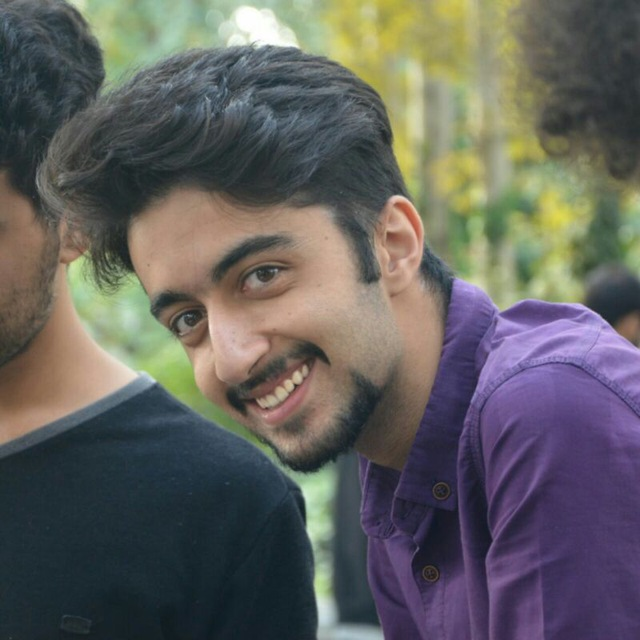
\includegraphics[width=3cm]{me.jpg}};
% \end{tikzpicture}
% \end{minipage} 
% \hfill
% %%%%%%%%%%%%%%%%%%%%%%%%%%%%%%%%%%%%% Image
\begin{minipage}[t]{0.40\textwidth} 
\vspace{10pt}
\begin{large}
	\headername{Behzad Shayegh Boroujeni}\\
\end{large}
\vspace{5pt}
University of Tehran, Tehran, Iran
\end{minipage} 
\hfill
\begin{minipage}[t]{0.35\textwidth} 
\vspace{20pt}
Mob.:\hfill +98-9381377391 \\
Email.:\hfill\textbf{\href{mailto:behzad.shayegh@ut.ac.ir}{behzad.shayegh@ut.ac.ir}} \\
Gmail.:\hfill\textbf{\href{mailto:behzad.shayegh.b@gmail.com}{behzad.shayegh.b@gmail.com}} \\
GitHub.:\hfill\textbf{\href{https://github.com/BehzadShayegh}{https://github.com/BehzadShayegh}} 
Web.:\hfill\textbf{\href{https://behzadshayegh.github.io}{https://behzadshayegh.github.io}} 
\end{minipage} 
\vspace{10pt}

%%%%%%%%%%%%%%%%%%%%%%%%%%%%%%%%%%%%%%
%
%     COLUMN ONE
%
%%%%%%%%%%%%%%%%%%%%%%%%%%%%%%%%%%%%%%

\begin{minipage}[t]{0.35\textwidth} 
%%%%%%%%%%%%%%%%%%%%%%%%%%%%%%%%%%%%%%
%     EDUCATION
%%%%%%%%%%%%%%%%%%%%%%%%%%%%%%%%%%%%%%
	My interest in natural language processing has encouraged me to gain knowledge and experience in this field. Also, I have work experience in feature extraction. Furthermore, I have good knowledge of algorithms, which positively affects my work experiences. In addition to my statistical knowledge, I am familiar with neural networks.
%%%%%%%%%%%%%%%%%%%%%%%%%%%%%%%%%%%%%%
%     EDUCATION
%%%%%%%%%%%%%%%%%%%%%%%%%%%%%%%%%%%%%%
\section{Education} 
\noindent\rule{5cm}{0.4pt}\\
\datecolor{2017-2022 (Expected)}
\subsection{Bachelor of Science}
\vspace{5pt}
\subsection{Major in Computer Engineering}
Software Engineering branch,\\
School of Electrical and Computer Engineering,
University of Tehran\\
GPA : 3.93/4 - 18.41/20 (till now)\\
\vspace{5pt}
\subsection{Minor in Computer Science}
School of Mathematics, Statistics and Computer Science,
University of Tehran\\
GPA : 4/4 - 19.73/20 (till now)\\

%%%%%%%%%%%%%%%%%%%%%%%%%%%%%%%%%%%%%%
%     COURSEWORK
%%%%%%%%%%%%%%%%%%%%%%%%%%%%%%%%%%%%%%
\section{Relevant Courses\\\vspace{-12pt}{\normalsize\normalfont (*: Graduate Course)}\vspace{-10pt}}
\noindent\rule{5cm}{0.4pt}\hfill Grade/20

Computational Neuroscience * \hfill 19.75 \\
\descriptright{\href{https://rtis2.ut.ac.ir/cv/mgtabesh/?lang=en-gb}{Assoc.Prof. Mohammad Ganjtabesh 
\includegraphics[width=8pt]{redirect.png}}}
Natural Language Processing * \hfill 19.1 \\
\descriptright{\href{https://ece.ut.ac.ir/en/~hfaili}{Assoc.Prof. Heshaam Faili 
\includegraphics[width=8pt]{redirect.png}}}
Reinforcement Learning * \hfill 20 \\
\descriptright{\href{https://ece.ut.ac.ir/en/~mnili}{Prof. Majid Nili 
\includegraphics[width=8pt]{redirect.png}}}
Statistical Machine Learning * \hfill 19.5 \\
\descriptright{\href{https://rtis2.ut.ac.ir/cv/z.rezaeigh/?lang=en-gb}{Assoc.Prof. Zahra Rezaei Ghahroodi 
\includegraphics[width=8pt]{redirect.png}}}
Artificial Intelligence\hfill 20 \\
\descriptright{\href{https://ece.ut.ac.ir/en/~asadeghi}{Assis.Prof. MohamadAmin Sadeghi 
\includegraphics[width=8pt]{redirect.png}}}
Statistical Methods\hfill 20 \\
\descriptright{Hasan Misaei}
Engineering Probability and Statistics\hfill 19.7 \\
\descriptright{\href{https://ece.ut.ac.ir/en/~Bahrak}{Assis.Prof. Behnam Bahrak 
\includegraphics[width=8pt]{redirect.png}}}
%%%%%%%%%%%%%%%%%%%%%%%%%%%%%%%%%%%%%%
%     Research Interests
%%%%%%%%%%%%%%%%%%%%%%%%%%%%%%%%%%%%%%
\section{Research Interests}
\noindent\rule{5cm}{0.4pt}
Computationl Neuroscience\\

\includegraphics[width=10pt]{subarrow.png} Spiking Neural Networks\\
Natural Language Processing\\

\includegraphics[width=10pt]{subarrow.png} Text Processing\\
Cybernetics\\

\includegraphics[width=10pt]{subarrow.png} Reinforcement Learning
\sectionsep
%%%%%%%%%%%%%%%%%%%%%%%%%%%%%%%%%%%%%%
%
%     COLUMN TWO
%
%%%%%%%%%%%%%%%%%%%%%%%%%%%%%%%%%%%%%%

\end{minipage} 
\hfill
\begin{minipage}[t]{0.6\textwidth} 
%%%%%%%%%%%%%%%%%%%%%%%%%%%%%%%%%%%%%%
%     Projects
%%%%%%%%%%%%%%%%%%%%%%%%%%%%%%%%%%%%%%
\section{Projects}
\noindent\rule{11.5cm}{0.4pt}
\datecolor{2021-now} \runsubsection{\href{https://github.com/BehzadShayegh/Spiral}{Spiking Neural Networks Framework}}
\descript{\href{https://github.com/BehzadShayegh/Spiral}{Spiral 
\includegraphics[width=8pt]{redirect.png}}}
\noindent
\hspace{5em}%
\begin{minipage}{0.85\textwidth\vspace{5pt}}
	\cvtag{Python}\cvtag{Compu-Neuro}\cvtag{SNN}\cvtag{PyTorch}\vspace{3pt}\\
	A python package for spiking neural network simulation using PyTorch on cuda or CPU.
	This package tries to bring its design as close as possible to biological observations of how the nervous system functions.
	It will be placed on the official website of the University of Tehran's Computational Neuroscience Research Lab shortly.\\
	\descriptright{\href{https://rtis2.ut.ac.ir/cv/mgtabesh/?lang=en-gb}{Supervisor: Assoc.Prof. Mohammad Ganjtabesh 
\includegraphics[width=8pt]{redirect.png}}}
\end{minipage}
\datecolor{2020-2021} \runsubsection{\href{https://behzadshayegh.github.io/PAT-github-pages/}{Persian Address to Postal-Code Convertor}}
\descript{\href{https://behzadshayegh.github.io/PAT-github-pages/}{PAT 
\includegraphics[width=8pt]{redirect.png}}}
\noindent
\hspace{5em}%
\begin{minipage}{0.85\textwidth\vspace{0pt}}
	\cvtag{Python}\cvtag{NLP}\cvtag{NLTK}\cvtag{Persian}\vspace{3pt}\\
	Persian Address Tracer (PAT) is an intelligent system for converting Persian text of address to postal code.
	If you are not aware, it is worth mentioning that due to the special conditions in the Persian language and
	also the lack of standards in addressing in Iran, this is a difficult issue.
	As far as we know, the PAT system is the most successful and intelligent system available for this issue.\\
	\descriptright{\href{https://ece.ut.ac.ir/en/~asadeghi}{Supervisor: Assis.Prof. MohamadAmin Sadeghi 
\includegraphics[width=8pt]{redirect.png}}}
\end{minipage}
%%%%%%%%%%%%%%%%%%%%%%%%%%%%%%%%%%%%%%
%     EXPERIENCE
%%%%%%%%%%%%%%%%%%%%%%%%%%%%%%%%%%%%%%
\section{Work Experience}
\noindent\rule{11.5cm}{0.4pt}
\datecolor{2019-2020} \runsubsection{\href{https://4choob.org/main-page}{House Prices Estimation over Tehran}}
\descript{\href{https://4choob.org/main-page}{4-Choob 
\includegraphics[width=8pt]{redirect.png}}}
\noindent
\hspace{5em}%
\begin{minipage}{0.85\textwidth\vspace{2pt}}
	\cvtag{Python}\cvtag{Numpy}\cvtag{Shapely}\cvtag{PostgreSQL}\cvtag{Q-GIS}\cvtag{PostGIS}\cvtag{Map-Processing}\vspace{3pt}\\
	4-Choob was a project aimed at automatic house price estimation over Tehran.
	The result of this project is a housing sales organization whose website is linked.
	We were the first members to work on this project and I was given the task of extracting features from multiple sources.
	The result was the extraction of more than 400 efficient price forecasting features.
	I used vary tools and techniques as there were very different tasks with different concerns;
	Such as map processing or optimization.\\
	\descriptright{\href{https://ece.ut.ac.ir/en/~asadeghi}{Supervisor: Assis.Prof. MohamadAmin Sadeghi 
\includegraphics[width=8pt]{redirect.png}}}
\end{minipage}
%%%%%%%%%%%%%%%%%%%%%%%%%%%%%%%%%%%%%%
%     BOOKs
%%%%%%%%%%%%%%%%%%%%%%%%%%%%%%%%%%%%%%
\section{Books}
\noindent\rule{11.5cm}{0.4pt}
\datecolor{2020-now} \runsubsection{\href{https://github.com/OpenBookshelf/DiscreteMathematics-Persian}{Discrete Mathematics Persian Book}}
\descript{\href{https://github.com/OpenBookshelf/DiscreteMathematics-Persian}{{\small OpenBookshelf} 
\includegraphics[width=7pt]{redirect.png}}}
\noindent
\hspace{5em}%
\begin{minipage}{0.85\textwidth\vspace{2pt}}
	\cvtag{LaTeX}\cvtag{Discrete-Mathematics}\vspace{3pt}\\
	I am the leader of a group of volunteers who are writing an Persian educational book on discrete mathematics.
	It is open-source and free for all.
	It is a charity act and everyone contributes without any expectations.
	FIPA will be registered soon.\\
	\descriptright{\href{https://ece.ut.ac.ir/en/~smohamadi}{Assoc.Prof. Siamak Mohammadi 
\includegraphics[width=8pt]{redirect.png}}}
\end{minipage}
\end{minipage}
\newpage
%%%%%%%%%%%%%%%%%%%%%%%%%%%%%%%%%%%%%%
%
%     Page 2
%
%%%%%%%%%%%%%%%%%%%%%%%%%%%%%%%%%%%%%%

%%%%%%%%%%%%%%%%%%%%%%%%%%%%%%%%%%%%%%
%     Teaching Assistance Experience
%%%%%%%%%%%%%%%%%%%%%%%%%%%%%%%%%%%%%%
\section{Teaching Assistance Experience}
\noindent\rule{11.5cm}{0.4pt}\\
\datecolor{Fall\;\;\;\; 2021} \runsubsection{\large Engineering Probability and Statistics (Head Teaching Assistant)}
\descript{\href{https://ece.ut.ac.ir/en/~Bahrak}{Assis.Prof. Behnam Bahrak 
\includegraphics[width=8pt]{redirect.png}}}
\vspace{3pt}
\noindent
\datecolor{Spring 2021}\\
\vspace{-3pt}
\datecolor{Fall\;\;\;\; 2020\;}\runsubsection{\large Discrete Mathematics (Head Teaching Assistant)}
\descript{\href{https://ece.ut.ac.ir/en/~smohamadi}{Assoc.Prof. Siamak Mohammadi 
\includegraphics[width=8pt]{redirect.png}}}
\vspace{-5pt}
\datecolor{Spring 2020}\\
\vspace{3pt}
\noindent
\datecolor{Spring 2021} \runsubsection{\large Natural Language Processing (Graduate Course)}
\descript{\href{https://ece.ut.ac.ir/en/~hfaili}{Assoc.Prof. Heshaam Faili 
\includegraphics[width=8pt]{redirect.png}}\\
\vspace{-5pt}\hfill\href{https://scholar.google.com/citations?user=TvGqaqAAAAAJ&hl=en}{Assis.Prof. Yadollah Yaghoobzadeh 
\includegraphics[width=8pt]{redirect.png}}}
\vspace{3pt}
\noindent
\datecolor{Spring 2020} \runsubsection{\large Artificial Intelligence}
\descript{\href{https://scholar.google.com/citations?user=zdY-omQAAAAJ&hl=en}{Dr. Hakimeh Fadaei 
\includegraphics[width=8pt]{redirect.png}}}
\vspace{3pt}
\noindent
\datecolor{Fall\;\;\;\; 2019} \runsubsection{\large Engineering Probability and Statistics}
\descript{\href{https://ece.ut.ac.ir/en/~Bahrak}{Assis.Prof. Behnam Bahrak 
\includegraphics[width=8pt]{redirect.png}}}
\vspace{3pt}
\noindent
\datecolor{Spring 2019\;}\runsubsection{\large Discrete Mathematics}
\descript{\href{https://ece.ut.ac.ir/en/~smohamadi}{Assoc.Prof. Siamak Mohammadi 
\includegraphics[width=8pt]{redirect.png}}}
\vspace{-5pt}
\datecolor{Fall\;\;\;\; 2019}\\
\vspace{3pt}
\noindent
\datecolor{Fall\;\;\;\; 2019} \runsubsection{\large Data Structures and Algorithms}
\descript{\href{https://ece.ut.ac.ir/en/~hfaili}{Assoc.Prof. Heshaam Faili 
\includegraphics[width=8pt]{redirect.png}}}
\vspace{3pt}
\noindent
\datecolor{Fall\;\;\;\; 2019} \runsubsection{\large  Introduction to Computing Systems and Programming}
\descript{\href{https://ece.ut.ac.ir/en/~moradih}{Assoc.Prof. Manouchehr MoradiSabzevar 
\includegraphics[width=8pt]{redirect.png}}}
\vspace{3pt}
\noindent
\datecolor{Fall\;\;\;\; 2018\;}\runsubsection{\large Engineering Programming}
\descript{\href{https://scholar.google.com/citations?user=TnZv6pkAAAAJ}{Dr. Noushin Karimian 
\includegraphics[width=8pt]{redirect.png}}}
\vspace{-5pt}
\datecolor{Spring 2018}\\
\vspace{7pt}
\noindent
{\Large Workshop Mentoring}
\noindent\rule{6.5cm}{0.4pt}\\
\vspace{3pt}
\datecolor{Spring\;\; 2020} \runsubsection{\large Python Tutorial}
\descript{Amirkabir University}
\noindent
\datecolor{Winter\; 2020} \runsubsection{\large Data Science Winter School}
\descript{Khatam University}
\noindent
\datecolor{Winter\; 2020} \runsubsection{\large Data Science Winter School}
\descript{University of Tehran}
\noindent
\datecolor{Summer 2019} \runsubsection{\large \href{https://github.com/BehzadShayegh/FraudDetection}{Summer of Code, AI Branch 
\includegraphics[width=8pt]{redirect.png}}}
\descript{University of Tehran}
\noindent

%%%%%%%%%%%%%%%%%%%%%%%%%%%%%%%%%%%%%%
%
%     COLUMN ONE
%
%%%%%%%%%%%%%%%%%%%%%%%%%%%%%%%%%%%%%%
\begin{minipage}[t]{0.48\textwidth}
	%%%%%%%%%%%%%%%%%%%%%%%%%%%%%%%%%%%%%%
	%     Written Contents
	%%%%%%%%%%%%%%%%%%%%%%%%%%%%%%%%%%%%%%
	\section{Written Contents} 
	
	\noindent\rule{9cm}{0.4pt}\\
	\datecolor{2021}
	\runsubsection{\large \href{https://colab.research.google.com/drive/1XY-6HmN6N2n2WMFHI2WUnYtVgcfm_02-}{Applied statistics tutorial in R 
\includegraphics[width=8pt]{redirect.png}}}\\
	\hfill
	\begin{minipage}{0.85\textwidth}
		\vspace{3pt}
		\normalsize
		- My Role: Leader\\
		- Usage: Engineering Probability and Statistics Course, School of Electrical and Computer Engineering, University of Tehran
	\end{minipage}\\
	\vspace{3pt}\descriptright{\href{https://ece.ut.ac.ir/en/~Bahrak}{Assis.Prof. Behnam Bahrak 
\includegraphics[width=8pt]{redirect.png}}}
	
	\datecolor{2020}
	\runsubsection{\large \href{https://github.com/soudabemhashemi/Common-Mistakes-in-Discrete-Mathematics}{Common Mistakes in Discrete Mathematics 
\includegraphics[width=8pt]{redirect.png}}}\\
	\hfill
	\begin{minipage}{0.85\textwidth}
		\vspace{3pt}
		\normalsize
		- My Role: Supervisor\\
		- Usage: Discrete Mathematics Course, School of Electrical and Computer Engineering, University of Tehran
	\end{minipage}\\
	\vspace{3pt}\descriptright{\href{https://ece.ut.ac.ir/en/~smohamadi}{Assoc.Prof. Siamak Mohammadi 
\includegraphics[width=8pt]{redirect.png}}}
	
	\datecolor{2020}
	\runsubsection{\large \href{https://github.com/BehzadShayegh/PythonTutorialExercises}{Python Tutorial Exercises 
\includegraphics[width=8pt]{redirect.png}}}\\
	\hfill
	\begin{minipage}{0.85\textwidth}
		\vspace{3pt}
		\normalsize
		- Usage: Python Tutorial in Amirkabir University
	\end{minipage}

	\datecolor{2018}
	\runsubsection{\large \href{https://github.com/BehzadShayegh/ExtraSolutionsAndCodes-44plus45}{ Extra Solutions And Codes (C++) Booklet 
\includegraphics[width=8pt]{redirect.png}}}\\
	\hfill
	\begin{minipage}{0.85\textwidth}
		\vspace{3pt}
		\normalsize
		- Usage: Computer Programming Course, Faculty of Engineering Sciences, University of Tehran
	\end{minipage}\\
	\vspace{3pt}\descriptright{\href{https://scholar.google.com/citations?user=TnZv6pkAAAAJ}{Dr. Noushin Karimian 
\includegraphics[width=8pt]{redirect.png}}}
\end{minipage}
%%%%%%%%%%%%%%%%%%%%%%%%%%%%%%%%%%%%%%
%
%     COLUMN TWO
%
%%%%%%%%%%%%%%%%%%%%%%%%%%%%%%%%%%%%%%
\hfill
\begin{minipage}[t]{0.48\textwidth}
	%%%%%%%%%%%%%%%%%%%%%%%%%%%%%%%%%%%%%%
	%     Python Packages
	%%%%%%%%%%%%%%%%%%%%%%%%%%%%%%%%%%%%%%
	\section{Python Packages} 
	\noindent\rule{9cm}{0.4pt}\\
	\datecolor{2021}
	\runsubsection{\large \href{https://pypi.org/project/add-on-class/}{Add-On Class 
\includegraphics[width=8pt]{redirect.png}}}\\
	
	\datecolor{2021}
	\runsubsection{\large \href{https://pypi.org/project/construction-requirements-integrator/}{Construction Requirements Integrator 
\includegraphics[width=8pt]{redirect.png}}}\\
	
	\datecolor{2021}
	\runsubsection{\large \href{https://pypi.org/project/matplotlib-dashboard/}{Matplotlib Dashboard 
\includegraphics[width=8pt]{redirect.png}}}\\
	
	\datecolor{2021}
	\runsubsection{\large \href{https://pypi.org/project/constant-properties-protector/}{Constant Properties Protector 
\includegraphics[width=8pt]{redirect.png}}}\\
\end{minipage}
\sectionsep
\newpage
%%%%%%%%%%%%%%%%%%%%%%%%%%%%%%%%%%%%%%
%
%     Page 3
%
%%%%%%%%%%%%%%%%%%%%%%%%%%%%%%%%%%%%%%

%%%%%%%%%%%%%%%%%%%%%%%%%%%%%%%%%%%%%%
%     SKILLS
%%%%%%%%%%%%%%%%%%%%%%%%%%%%%%%%%%%%%%
\section{Skills}
\noindent\rule{9cm}{0.4pt}\vspace{10pt}\\
	\begin{tabular}{ c c c c c c }
				& {Programming} 						& {Python Libraries} 						& {Software} 								& {Other Tools} 						\\
				& {Languages}   						& {\& Frameworks}    						& {\& DBMSs} 								& {\& Frameworks} 						\vspace{7pt}\\
	{Expert}    & \cvtag{Python}\cvtag{TeX}\cvtag{SQL} 	& \cvtag{Pandas}\cvtag{Numpy}\cvtag{Spiral}	& \cvtag{Git}\cvtag{LaTeX}\cvtag{PostgreSQL}& \cvtag{Spreadsheet}\cvtag{Markdown}	\vspace{7pt}\\
	{Proficient}& \cvtag{R}\cvtag{Bash} 				& \cvtag{PyTorch}\cvtag{Matplotlib}			& \cvtag{MySQL}\cvtag{PostGIS}				& \cvtag{HTML}\cvtag{CSS}				\\
				& 						 				& \cvtag{NLTK}\cvtag{Scikit-Learn}			& 											& \cvtag{Jupyter}\cvtag{Colab}			\vspace{7pt}\\
	{Familiar} 	& \cvtag{C++}\cvtag{C}\cvtag{Java} 		& \cvtag{Keras}\cvtag{BindsNET} 			& \cvtag{Q-GIS}								& \cvtag{ReactJS}\cvtag{VueJS}			\\
			 	& \cvtag{Verilog}\cvtag{JavaScript} 	& \cvtag{Shapely}\cvtag{SciPy.stats}  		&											& 										\vspace{7pt}\\
	{Beginner} 	& \cvtag{MATLAB}\cvtag{C\#}				& \cvtag{Sympy} 							& \cvtag{MongoDB}\cvtag{Elasticsearch}		& \cvtag{Spring}						\\
	\end{tabular}
\sectionsep
%%%%%%%%%%%%%%%%%%%%%%%%%%%%%%%%%%%%%%
%     Notable Course Projects
%%%%%%%%%%%%%%%%%%%%%%%%%%%%%%%%%%%%%%
\section{Notable Course Projects}
\noindent\rule{11.5cm}{0.4pt}\\
\datecolor{Spring 2021} \runsubsection{\large \href{https://github.com/BehzadShayegh/Text-Representation-using-Recurrent-Spiking-Neural-Networks}{Text Representation using SNNs (to be continued) 
\includegraphics[width=8pt]{redirect.png}}}
\descript{Computationl Neuroscience\\
\vspace{-5pt}\hfill\href{https://rtis2.ut.ac.ir/cv/mgtabesh/?lang=en-gb}{Assoc.Prof. Mohammad Ganjtabesh 
\includegraphics[width=8pt]{redirect.png}}}
\vspace{3pt}
\noindent
\datecolor{Spring 2021} \runsubsection{\large \href{https://github.com/BehzadShayegh/Face-Representation-using-Convolutional-SNNs}{Face Representation using Convolutional SNNs 
\includegraphics[width=8pt]{redirect.png}}}
\descript{Natural Language Processing\\
\vspace{-5pt}\hfill\href{https://ece.ut.ac.ir/en/~hfaili}{Assoc.Prof. Heshaam Faili 
\includegraphics[width=8pt]{redirect.png}}}
\vspace{3pt}
\noindent
\datecolor{Spring 2020} \runsubsection{\large \href{https://github.com/BehzadShayegh/SpamDitection-IMDB-Using-Bert-Elmo}{IMDB Spam Ditection using Bert and Elmo 
\includegraphics[width=8pt]{redirect.png}}}
\descript{Natural Language Processing\\
\vspace{-5pt}\hfill\href{https://ece.ut.ac.ir/en/~hfaili}{Assoc.Prof. Heshaam Faili 
\includegraphics[width=8pt]{redirect.png}}}
\vspace{3pt}
\noindent
\datecolor{Spring 2020} \runsubsection{\large \href{https://github.com/BehzadShayegh/POS-Tagging}{POS Tagging using RNN and HMM 
\includegraphics[width=8pt]{redirect.png}}}
\descript{Natural Language Processing\\
\vspace{-5pt}\hfill\href{https://ece.ut.ac.ir/en/~hfaili}{Assoc.Prof. Heshaam Faili 
\includegraphics[width=8pt]{redirect.png}}}
\vspace{3pt}
\noindent
\datecolor{Spring 2020} \runsubsection{\large \href{https://github.com/BehzadShayegh/NeuralMachineTranslation}{Fa2En and En2Fa Neural Machine Translation 
\includegraphics[width=8pt]{redirect.png}}}
\descript{Natural Language Processing\\
\vspace{-5pt}\hfill\href{https://ece.ut.ac.ir/en/~hfaili}{Assoc.Prof. Heshaam Faili 
\includegraphics[width=8pt]{redirect.png}}}
\vspace{3pt}
\noindent
\datecolor{Spring 2020} \runsubsection{\large \href{https://github.com/BehzadShayegh/FeedForwardNeuralNetworkLanguageModel}{Feed Forward Neural Network Language Model \includegraphics[width=8pt]{redirect.png}}}
\descript{Natural Language Processing\\
\vspace{-5pt}\hfill\href{https://ece.ut.ac.ir/en/~hfaili}{Assoc.Prof. Heshaam Faili \includegraphics[width=8pt]{redirect.png}}}
\vspace{3pt}
\noindent
\datecolor{Spring 2020} \runsubsection{\large \href{https://github.com/BehzadShayegh/MovieReviewsSemanticAnalysis}{Movie Reviews Semantic Analysis using Statistical Language Models \includegraphics[width=8pt]{redirect.png}}}
\descript{Natural Language Processing\\
\vspace{-5pt}\hfill\href{https://ece.ut.ac.ir/en/~hfaili}{Assoc.Prof. Heshaam Faili \includegraphics[width=8pt]{redirect.png}}}
\vspace{3pt}
\noindent
\datecolor{Spring 2020} \runsubsection{\large \href{https://github.com/BehzadShayegh/NewsClassification}{Persian News Classification using Statistical Language Models \includegraphics[width=8pt]{redirect.png}}}
\descript{Natural Language Processing\\
\vspace{-5pt}\hfill\href{https://ece.ut.ac.ir/en/~hfaili}{Assoc.Prof. Heshaam Faili \includegraphics[width=8pt]{redirect.png}}}
\vspace{3pt}
\noindent
\datecolor{Spring 2019} \runsubsection{\large \href{https://github.com/BehzadShayegh/SpamDitection}{Emails Spam Detection using Bag of Words \includegraphics[width=8pt]{redirect.png}}}
\descript{Artificial Intelligence\\
\vspace{-5pt}\hfill\href{https://ece.ut.ac.ir/en/~asadeghi}{Assis.Prof. MohamadAmin Sadeghi \includegraphics[width=8pt]{redirect.png}}}
\vspace{3pt}
\noindent
\datecolor{Spring 2019} \runsubsection{\large \href{https://github.com/BehzadShayegh/CIFAR10-CNN}{Image Classification (CIFAR-10) using CNNs \includegraphics[width=8pt]{redirect.png}}}
\descript{Artificial Intelligence\\
\vspace{-5pt}\hfill\href{https://ece.ut.ac.ir/en/~asadeghi}{Assis.Prof. MohamadAmin Sadeghi \includegraphics[width=8pt]{redirect.png}}}
\vspace{3pt}
\noindent
\datecolor{Spring 2019} \runsubsection{\large \href{https://github.com/BehzadShayegh/MNIST-CIFAR10_ScikitLearn}{Image Classification (MNIST and CIFAR-10) using ML approachs \includegraphics[width=8pt]{redirect.png}}}
\descript{Artificial Intelligence\\
\vspace{-5pt}\hfill\href{https://ece.ut.ac.ir/en/~asadeghi}{Assis.Prof. MohamadAmin Sadeghi \includegraphics[width=8pt]{redirect.png}}}
\vspace{3pt}
\noindent
\datecolor{Spring 2019} \runsubsection{\large \href{https://github.com/BehzadShayegh/ZillowPrize1}{House Price Estimation using Neural Networks \includegraphics[width=8pt]{redirect.png}}}
\descript{Artificial Intelligence\\
\vspace{-5pt}\hfill\href{https://ece.ut.ac.ir/en/~asadeghi}{Assis.Prof. MohamadAmin Sadeghi \includegraphics[width=8pt]{redirect.png}}}
\vspace{3pt}
\noindent
{\Large Hands-On Series}
\noindent\rule{7cm}{0.4pt}\\
\datecolor{Spring 2021} \runsubsection{\large \href{https://github.com/BehzadShayegh/Assignments-CNS-Spring2021}{Understand the parameters in SNNs (9 Parts) \includegraphics[width=8pt]{redirect.png}}}
\descript{Computationl Neuroscience\\
\vspace{-5pt}\hfill\href{https://rtis2.ut.ac.ir/cv/mgtabesh/?lang=en-gb}{Assoc.Prof. Mohammad Ganjtabesh \includegraphics[width=8pt]{redirect.png}}}
\vspace{3pt}
\noindent
\datecolor{Fall\;\;\;\; 2020} \runsubsection{\large \href{https://github.com/BehzadShayegh/Assignments-RL-Fall2020}{Apply well-known RL algorithms on simulated problems (5 Parts) \includegraphics[width=8pt]{redirect.png}}}
\descript{Reinforcement Learning\\
\vspace{-5pt}\hfill\href{https://ece.ut.ac.ir/en/~mnili}{Prof. Majid Nili \includegraphics[width=8pt]{redirect.png}}}
\vspace{3pt}
\noindent
\datecolor{Fall\;\;\;\; 2020} \runsubsection{\large \href{https://github.com/BehzadShayegh/Assignments-SML-Fall2020}{Statistical analysis on datasets and ML models performance(5 Parts) \includegraphics[width=8pt]{redirect.png}}}
\descript{Statistical Machine Learning\\
\vspace{-5pt}\hfill\href{https://rtis2.ut.ac.ir/cv/z.rezaeigh/?lang=en-gb}{Assoc.Prof. Zahra Rezaei Ghahroodi \includegraphics[width=8pt]{redirect.png}}}
\noindent
%%%%%%%%%%%%%%%%%%%%%%%%%%%%%%%%%%%%%%
%
%     COLUMN ONE
%
%%%%%%%%%%%%%%%%%%%%%%%%%%%%%%%%%%%%%%
\begin{minipage}[t]{0.33\textwidth}
	%%%%%%%%%%%%%%%%%%%%%%%%%%%%%%%%%%%%%%
	%     Languages
	%%%%%%%%%%%%%%%%%%%%%%%%%%%%%%%%%%%%%%
	\section{Languages}
	\noindent\rule{6.5cm}{0.4pt}\vspace{4pt}\\
	Persian \hfill . . . . . . . . . \hfill Native\\
	\vspace{5pt}
	English \hfill . . . . . . . . . \hfill Fluent\\
	‌\hspace{33pt}\includegraphics[width=10pt]{subarrow.png} IELTS Score: Overal: 6.5 \\
	‌\hfill R: 6.5 | L: 6.5 | S: 6.5 | W: 6.5
\end{minipage}
%%%%%%%%%%%%%%%%%%%%%%%%%%%%%%%%%%%%%%
%
%     COLUMN TWO
%
%%%%%%%%%%%%%%%%%%%%%%%%%%%%%%%%%%%%%%
\hfill
\begin{minipage}[t]{0.6\textwidth}
	%%%%%%%%%%%%%%%%%%%%%%%%%%%%%%%%%%%%%%
	%     Refrences
	%%%%%%%%%%%%%%%%%%%%%%%%%%%%%%%%%%%%%%
	\section{Refrences} 
	\noindent\rule{9cm}{0.4pt}\\
\end{minipage}

\end{document}  \documentclass[]{article}